\chapter{Wprowadzenie}
\label{cha:wprowadzenie}
Morfologia krwi jest jednym z najczęściej przeprowadzanych badań. Zgodnie z zaleceniami powinno się wykonywać je przynajmniej raz do roku. Według reportu GUS 42\% osób decydujących się na badanie labolatoryjne wybiera właśnie badanie krwi \cite{GUS_Zdrowie2016}. Biorąc pod uwagę stan ludności i ograniczoną liczbę personelu medycznego w szpitalach maualne wykonywanie tego typu badań jest problematyczne i zajmuje dużo czasu, który można oszczędzić przeprowadzając automatyzację tego procesu.

\begin{figure}[h]
	\centering
		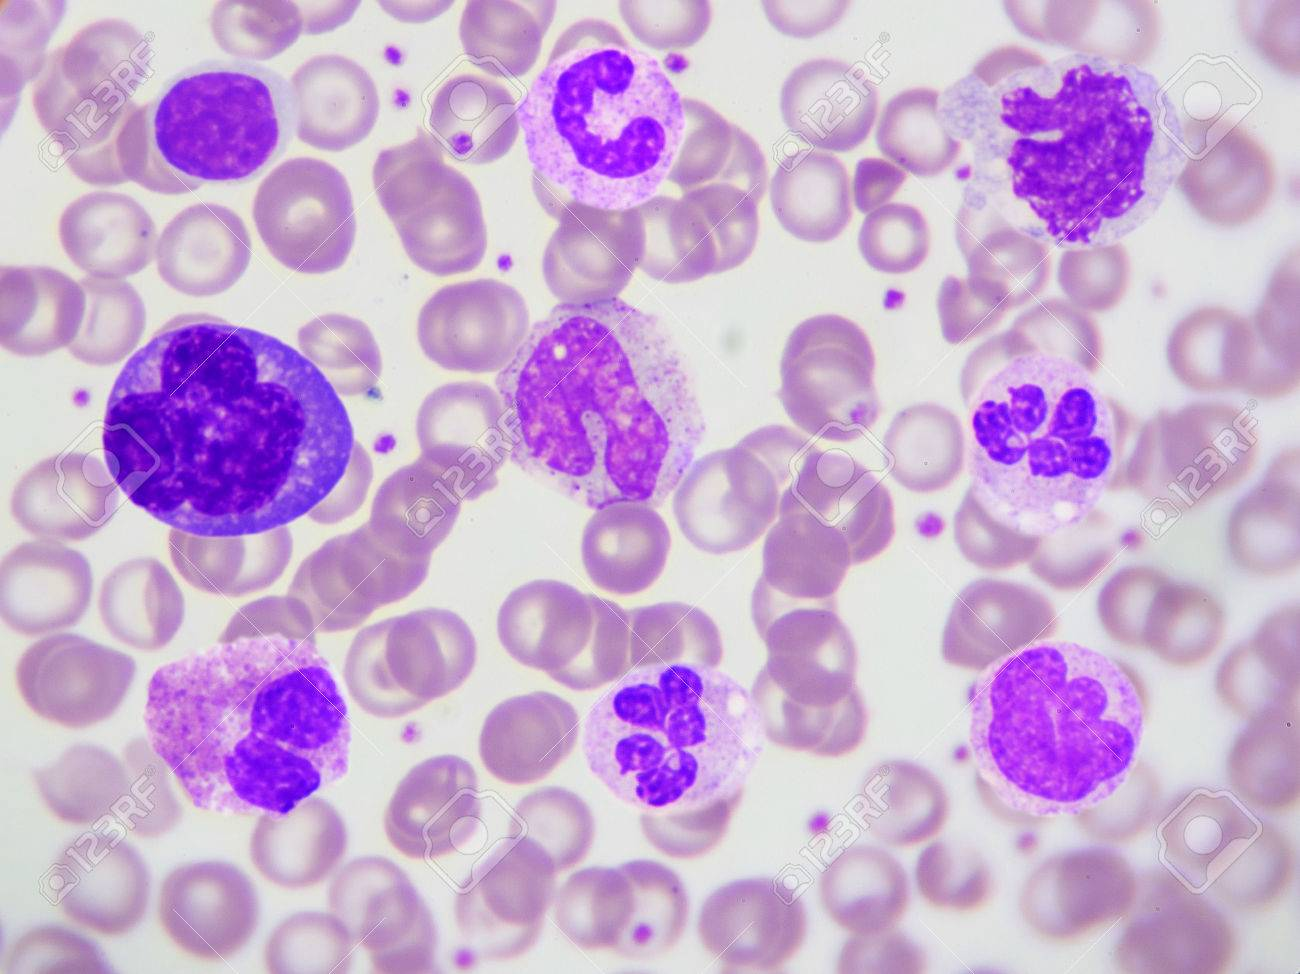
\includegraphics[scale=0.60]{blood_cells_microscope}
	\caption{Widok krwinek badanych pod mikroskopem \cite{cells_microscope}.}
\end{figure}

Celem pracy jest zbudowanie narzędzia do klasyfikacji białych krwinek opartego na głęboko uczonych konwolucyjnych sieciach neuronowych. Na wejściu do sieci wprowadzane są zdjęcia pojedynczych krwinek, wykonane pod mikroskopem. W tym celu została wykorzystana baza danych na licencji MIT, zawierająca cztery klasy krwinek najliczniej występujące w składzie krwi. Każde zdjęcie jest oryginalnie przyporządkowane do odpowiedniej klasy, zgodnie z widniejącym na nim elementem morfologicznym. 

Przed użyciem bazę podzielono na rozłączne zbiory: uczący, weryfikacyjny i testowy. Za pomocą zbiorów uczącego i weryfiacyjnego przetrenowano i nastrojono klasyfikator. Dzięki danym ze zbioru testowego zawierającego zdjęcia nigdy nie wprowadzane na wejście sieci sprawdzono skuteczność zastosowanej metody.

Oczekiwanym wynikiem pracy jest zbudowanie sieci neuronowej określającej z jak najlepszą doładnośćią jaki typ krwinki znajduje się na zdjęciu, a następnie modyfikacja zarówno parametrów sieci jak i danych wejściowych w celu zbadania wpływu zmian na działanie modelu.

Program został napisany w języku Python, który jest dobrze przystosowany do przetwarzania, analizy i modelowania danych. Do implementacji sieci użyta została biblioteka Keras, która jest wysokopoziomowym API biblioteki TensorFlow.

%---------------------------------------------------------------------------
\section{Motywacja pracy}
\label{sec:motywacja_pracy}

W celu prawidłowego zdiagnozowania chorób często konieczne jest zbadanie liczby krwinek białych danego typu. Obecnie proces ten jest wykonywany manualnie za pomocą hemocymetru lub automatycznie z użyciem np. technologii VCS, pomiarem impedancji czy pomiarami z użyciem laseru. 

Ciekawą alternatywą dla tych metod byłoby zastosowanie zliczania w czasie rzeczywistym komórek opartego na klasyfikacji przynależności do danego typu na podstawie analizy obrazów przez sieć neuronową. Byłaby to metoda nie wymagająca ingerencji czynnika ludzkiego, jak to ma miejsce w przypadku badania manualnego, a jednocześnie tańsza niż stosowane pomiary automatyczne.

Bazą do zbudowania tego typu narzędzia byłaby sieć rozpoznająca typ krwinki na zdjęciu i właśnie tą częścią zajmuje się niniejszy projekt. W pracy zdecydowano się na sieć konwolucyjną głęboko uczoną i w zależności od parametrów zbadano precyzyjność jej działania. W tym celu przetestowano wiele kombinacji doboru składowych modelu, a poniżej opisano kilka najciekawszych przypadków.

%---------------------------------------------------------------------------

\section{Zawartość pracy}
\label{sec:zawartoscPracy}

W rodziale~\ref{cha:teoria} przedstawiono teoretyczną analizę problemu badawczego wraz z kilkoma przykładowymi rozwiązaniami zadania klasyfikacji wizyjnej na podstawie najnowszych publikacji.

%Analiza problemu badawczego: opis zagadnień związanych z analizowanym problemem. Rozdział powinien składać się z dwóch podrozdziałów. Pierwszy podrozdział analizuje problem badawczy od strony technicznej/medycznej, drugi podrozdział podstawy techniczne/implementacyjne. Rozwinięcie wstępu jak również podstawy dla następnych rozdziałów umożliwiające ich zrozumienie.

Rozdział ~\ref{cha:autorskie} zawiera opis implementacji programu i zastosowanych metod, po którym następuje krótkie podsumowanie uzyskanych wyników. 
%Od rozdziału 3 przedstawiamy już tylko autorskie rozwiązanie + opis zastosowanych metod. Iplementacja projektu, co zostało zaimplementowane, jak zostało zaimplementowane, jak zostały spełnione wymagania, napotkane problemy i ich rozwiązania.
%Wyniki i ich opracowanie, przeprowadzone testy.
%Podsumowanie: przypomniec cel pracy, jak zostały spełnione wymagania: implikacje, konsekwencje, walory, w jaki sposób zaimplementowana technologia rozwiązuje postawione problemy,czy wszystkie problemy zostały rozwiązane,jakie nie zostały rozwiązane, dlaczego?
%Bibliografia.
%Opcjonalne załączniki.

%Z bazy:
%Celem pracy inżynierskiej jest zaproponowanie rozwiązania bazującego na głębokich sieciach neuronowych do klasyfikacji 4 typów białych krwinek-leukocytów (ang. white blood cells). Proponowana jest sieć konwolucyjna z odpowiednim doborem hiperparametrów, funkcji aktywacji oraz warstw. Rozwiązanie zostanie zaimplementowane w języku Python z wykorzystaniem biblioteki Tensorflow. 
